% $Id: CoreClasses.tex,v 1.1 2008/01/31 18:04:16 dconway Exp $
\chapter{\label{chapter:CoreClasses}The GmatBase Class, Constants, and Defined Types}
\chapauthor{Darrel J. Conway}{Thinking Systems, Inc.}

This chapter documents GMAT's predefined data types, constants, and the core user classes used in
GMAT to implement the flight dynamics model.

\section{Defined Data Types}

GMAT uses the C++ type definition mechanism to define the data types shown in
Table~\ref{table:GmatDataTypes}.  These definitions, found in the gmatdefs.hpp header file, provide
a mechanism to generalize common data types and frequently used structures in the source code.

\begin{table}[H]
\begin{center}
\caption{\label{table:GmatDataTypes}Data Types Defined for GMAT}
\setlength\extrarowheight{2pt}
\begin{tabular}{|p{2in}|p{1.2in}|p{2.5in}|}
\hline
Defined typedef & Type Name & Description \\
\hline
\hline
double & Real & 8 byte float\\
int & Integer & 4 byte signed integer\\
unsigned char & Byte & 1 byte character\\
unsigned int & UnsignedInt & 4 byte unsigned integer\\
std::vector<Real> & RealArray & Vector of Reals\\
std::vector<Integer> & IntegerArray & Vector of signed integers\\
std::vector<UnsignedInt> & UnsignedIntArray & Vector of unsigned integers\\
std::vector<std::string> & StringArray & Vector of strings\\
std::vector<GmatBase*> & ObjectArray & Vector of GmatBase objects\\
std::vector<Gmat::ObjectType> & ObjectTypeArray & Vector of object type identifiers\\
\hline
\end{tabular}
\end{center}
\end{table}

\section{Error Handling in GMAT}

GMAT responds to critical anomalies in the configuration or other settings by throwing exceptions
reporting the error.  Every effort has been made to make GMAT's exception messages consistent and
informative.  Less serious anomalies may be reported through masseges passed as warnings to GMAT's
messaging system.  The classes implemented to support these two mechanisms are documented in
Chapter~\ref{chapter:Utilities}.

\section{\label{section:GmatBase}GmatBase}

The factory classes described in Chapter~\ref{chapter:Factories} are used to generate the resources
and Mission Control Sequence commands needed to simulate flight dynamics models.  The objects that
are generated in GMAT corresponding to these model elements are all instances of classes derived
from a base class named GmatBase.  The GmatBase class defines a common set of interfaces used to
build, configure, maintain, and store these elements.  This commonality of the interfaces into user
defined objects enforces consistency, simplifying common tasks that are performed on these objects.

Since understanding of the GmatBase is key to understanding how to work with the source code for
the model, this section of the document is written to thoroughly capture the contents of the class.
We'll begin by examining the class features in the following sections, and then provide some
information about how GMAT uses these features to set properties while reading and to serialize
model objects while writing objects to a text stream.

\subsection{GmatBase Attributes and Methods}

The features of GmatBase are broken into the class attributes and methods.  The method descriptions
are categorized into ??? subsections: (1) Constructors, Destructor, and Static Methods, (2) Object
Management Interfaces, (3) Interfaces Used for Scripting, the GUI, and External Communications, (4)
Class Attributes for Referenced and Owned Objects, (5) Class Attribute Management interfaces, and
(6 -- 9) sections for the interfaces into Reals, Integers, Strings, and other attribute types.

\subsubsection{\textit{Class Attributes}}

GmatBase contains data structures designed to manage the common elements shared by all of the
derived classes.  Configurable pieces of the derived classes are referred to as ``parameters'' in
the GmatBase code; hence the Integer attribute ``parameterCount'' reports the number of parameters
that can be accessed for instances of the derived class.  The attributes of GmatGase are described
here:

\begin{itemize}
\item \textbf{static Integer instanceCount}: Count of the number of GmatBase objects currently
instantiated.
\item \textbf{Integer parameterCount}: Count of the accessible parameters.
\item \textbf{std::string typeName}: Script string used or this class.
\item \textbf{std::string instanceName}: Name of the object -- empty if it is nameless.
\item \textbf{Gmat::ObjectType type}: Enumerated base type of the object.
\item \textbf{Integer ownedObjectCount}: Number of owned objects that belong to this instance.
\item \textbf{std::string generatingString}: Script string used to build the object.
\item \textbf{ObjectTypeArray objectTypes}: The list of generic types that this class extends.
\item \textbf{StringArray objectTypeNames}: The list types that this class extends, by name.
\item \textbf{ObjectTypeArray refObjectTypes}: The list of object types referenced by this class.
\item \textbf{StringArray refObjectNames}: The list of object names referenced by this class.
\item \textbf{bool callbackExecuting}: Flag indicating whether or not a Callback method is currently
executing.
\item \textbf{std::string errorMessageFormat}: The format string used when throwing error messages
for named objects.
\item \textbf{std::string errorMessageFormatUnnamed}: The format string used when throwing error
messages for unnamed objects.
\item \textbf{bool inMatlabMode}: Flag used to deterine if the current write is in Matlab mode.
\item \textbf{std::string commentLine}: String used to hold the comment line.
\item \textbf{std::string inlineComment}: String used to hold inline comment.
\item \textbf{StringArray attributeCommentLines}: String array used to hold the attribute comments.
\item \textbf{StringArray attributeInlineComments}: String array used to hold the attribute inline
comments.
\end{itemize}

\subsubsection{\textit{Constructor, Destructor, and Static Methods}}

GmatBase implements methods that override the default compiler-generated construction and
destruction capabilities, along with several class level utilities, as described below.

\paragraph{Default Methods}

C++ automatically defines four methods when a class is defined in code: a default constructor, a
copy constructor, a destructor, and an assignment operator.  Every user class in GMAT overrides
these methods to prevent generation of the default compiler versions.

\begin{itemize}
\item \textbf{GmatBase(Gmat::ObjectType typeId, const std::string \&typeStr, const std::string
\&nomme = "")}:  This is the default constructor for all GmatBase objects.
\item \textbf{virtual ~GmatBase() = 0}:  The base class destructor.  The destructor is set as
abstract, but it does have an implementation; designating it as abstract ensures that the compiler
will not allow GmatBase base class instances.
\item \textbf{GmatBase(const GmatBase \&a)}: The copy constructor.
\item \textbf{GmatBase\& operator=(const GmatBase \&a)}:  The assignment operator.
\end{itemize}

\paragraph{Static Methods}

The GmatBase class provides a mechanism to count object instances, provide numerical precision
setting data, and find object types and names through the following static class methods:

\begin{itemize}
\item \textbf{static Integer GetInstanceCount()}: Method to return the current number of
instantiated objects.
\item \textbf{static Integer GetDataPrecision()}: Returns the current precision setting used when
converting Real numbers into strings.
\item \textbf{static Integer GetTimePrecision()}: Returns the current precision setting used when
converting epoch data into strings.
\item \textbf{static std::string GetObjectTypeString(Gmat::ObjectType type)}: Method for getting
GMAT object type string.
\item \textbf{static Gmat::ObjectType GetObjectType(const std::string \&typeString)}: Method for
getting GMAT object type.
\end{itemize}

\subsubsection{\textit{Object Management Interfaces}}

GmatBase provides interfaces that are used to identify the object so that it can be accessed, and so
that other objects can find and connect to it.  These interfaces are described in this section.

\paragraph{Base Class Property Interfaces}

We'll begin by listing the interfaces that are used to retrieve information about the current
object.

\begin{itemize}
\item \textbf{virtual Gmat::ObjectType GetType() const}: Retrieves the core type of the object.
\item \textbf{inline std::string GetTypeName() const}: Retrieves the test description used for the
object type.
\item \textbf{inline std::string GetName() const}: Retrieves teh object's name.  Names in GMAT are
used to access objects in the Configuration; each user defined object that is stored in the
configuration is given a unique name.
\item \textbf{virtual bool SetName(const std::string \&who, const std::string \&oldName = "")}:
Renames the object.
\item \textbf{virtual Integer GetParameterCount() const}: Returns the number of parameters that can
be accessed for the object using the parameter interfaces, discussed below.
\item \textbf{bool IsOfType(Gmat::ObjectType ofType)}: Checks the object to see if it is derived
from the specified ObjectType.
\item \textbf{bool IsOfType(std::string typeDescription)}: Checks the object to see if it is derived
from the specified named type.
\end{itemize}

\paragraph{Overridable Interfaces}

The interfaces listed next are interfaces that are overrridden in the derived classes to provide
functionality as needed.

\begin{itemize}
\item \textbf{virtual GmatBase* Clone() const = 0}: Every GmatBase derived class that can be
instantiated must implement the Clone() method.  Clone() is used to copy objects from the
configuration into the Sandbox prior to the execution of the Mission Control Sequence.
\item \textbf{virtual void Copy(const GmatBase*)}: The Copy() method is provided so that objects
that need to copy data from other objects of the same class type can do so even when referenced
through GmatBase pointers.
\item \textbf{virtual bool Initialize()}: Objects that need to preform specific initialization
tasks override this method to perform those tasks.  The Sandbox calls the Initialize() method as
part of the Sandbox initialization process.
\item \textbf{virtual void SetSolarSystem(SolarSystem *ss)}: Objects that need access to GMAT's
current SolarSystem object override this method to set their SolarSystem pointer.
\item \textbf{virtual bool RequiresJ2000Body()}: Classes that need location data in the model use a
referenced body -- referred to as the J2000 body -- as the origin for spatial conversions.  Classes
that require this body override the RequiresJ2000Body method to return true from this call.
\item \textbf{virtual bool TakeAction(const std::string \&action, const std::string \&actionData =
"")}:  TakeAction() is a utility method that derived classes override to provide functionality that
cannot be implemented through basic parameter setting calls\footnote{One example of the use of the
TakeAction() can be found in the Spacecraft class.  The Spacecraft class uses TakeAction() to
manage attached tank and thruster objects.  Tanks and Thrusters are attached by name to the
Spacecraft instances during configuration, but the actual member objects are set during Sandbox
initialization through a call, ``TakeAction("SetupHardware");'', made to the Spacecraft object.}.
\item \textbf{virtual void FinalizeCreation()}: Performs initialization of GmatBase properties that
depend on the features of the derived classes.  Derived classes can touch some of the base class
properties -- the parameterCount, for example.  This method is called after the object creation
process is complete, so that any of the object's base-class properties can be updated to reflect
the object's actual properties.
\item \textbf{virtual std::string GetErrorMessageFormat()}: Returns the error message format string
used by the object.
\item \textbf{virtual void SetErrorMessageFormat(const std::string \&fmt)}: Updates the error
message format string used by the object.
\end{itemize}

\subsubsection{\textit{Interfaces Used for Scripting, the GUI, and External Communications}}

The interfaces used for scripting and callbacks are described in the following paragraphs.

\paragraph{General Purpose Interfaces}

All of the objects used in GMAT's model have the ability to produce text descriptions -- aka script
blocks -- sufficient to reproduce themselves and to incorporate text comments that help document the
intent of the setting selected by the user.  These interfaces are described here:

\begin{itemize}
\item \textbf{virtual const std::string GetCommentLine() const}: Returns the comment lines that
occur before the object definition or command line.
\item \textbf{virtual void SetCommentLine(const std::string \&comment)}: Sets the comment lines that
occur before the object definition or command line.
\item \textbf{virtual const std::string GetInlineComment() const}: Returns the comment that occurs
inline at the end of the object definition or command line.
\item \textbf{virtual void SetInlineComment(const std::string \&comment)}: Sets the comment that
occurs inline at the end of the object definition or command line.
\item \textbf{virtual const std::string GetAttributeCommentLine(Integer index)}: Returns any comment
that occurs before an attribute setting line.
\item \textbf{virtual void SetAttributeCommentLine(Integer index, const std::string \&comment)}:
Sets a comment that occurs before the attribute setting line.
\item \textbf{virtual const std::string GetInlineAttributeComment(Integer index)}: Returns the
comment that occurs at the end of an attribute setting line.
\item \textbf{virtual void  SetInlineAttributeComment(Integer index, const std::string \&comment)}:
Sets the comment that occurs at the end of an attribute setting line.
\item \textbf{virtual const std::string\& GetGeneratingString(Gmat::WriteMode mode =
Gmat::SCRIPTING, const std::string \&prefix = "", const std::string \&useName = "")}: Returns a
text string that can be used to regenerate the object.  See Section~\ref{section:GenStringModes} for
an explanation of the write modes.
\item \textbf{virtual StringArray GetGeneratingStringArray(Gmat::WriteMode mode = Gmat::SCRIPTING,
const std::string \&prefix = "", const std::string \&useName = "")}: Returns a string array that can
be used to regenerate the object.  See Section~\ref{section:GenStringModes} for an explanation of
the write modes.
\item \textbf{void CopyParameters(const GmatBase \&a)}: Copies the attributes from one object into
the current object.
\item \textbf{virtual void WriteParameters(Gmat::WriteMode mode, std::string \&prefix,
std::stringstream \&stream)}: Writes the parameter details for an object.  This method is called by
the GetGeneratingString methods to build the individual attribute lines needed to write configured
objects.
\item \textbf{void WriteParameterValue(Integer id, std::stringstream \&stream)}: Formats and
writes the attribute value portion of the attribute line.
\item \textbf{virtual void PrepCommentTables()}: A private method used to configure teh comment
tables so that they are sized correctly for the owning object.
\end{itemize}

\paragraph{Callback Interfaces}

Some GMAT classes are designed to communicate with external process through a basic callback
method.  These classes override the following methods to implement callbacks.

\begin{itemize}
\item \textbf{virtual bool ExecuteCallback()}: The method called from the external process to
execute a task in GMAT.
\item \textbf{virtual bool IsCallbackExecuting()}: Monitoring function used to determine if the
object is executing its callback method.
\item \textbf{virtual bool PutCallbackData(std::string \&data)}: Sends data from GMAT to the process
that is using the callback.
\item \textbf{virtual std::string GetCallbackResults()}: Retrieves the results of the callback.
\end{itemize}

\subsubsection{\textit{Class Attributes: Referenced and Owned Objects}}

Many of the user created objects need to interact with other model objects to correctly model the
spacecraft mission.  When an object uses the interfaces for a second named object that is stored in
the configuration, the second object is called a ``referenced object'' in this document. 
Occasionally an object will have, as a wholly owned, encapsulated member, another object.  These
internal member objects are called ``owned objects.''  The methods listed here are implemented to
work with the owned and referenced objects.

\begin{itemize}
\item \textbf{virtual std::string GetRefObjectName(const Gmat::ObjectType type) const}: Returns the
name of a referenced object of a specified type, of the object uses that type of referenced object.
\item \textbf{virtual const ObjectTypeArray\& GetRefObjectTypeArray()}: Returns an array of the
reference object types used by the current object.  Derived classes set the types in the
refObjectTypes attribute, which is returned from this call.
\item \textbf{virtual const StringArray\& GetRefObjectNameArray(const Gmat::ObjectType type)}:
Returns the reference object names used by the current object.  Derived classes override this
method to return the correct values.
\item \textbf{virtual bool SetRefObjectName(const Gmat::ObjectType type, const std::string
\&name)}: Sets the name of a referenced object.
\item \textbf{virtual bool RenameRefObject(const Gmat::ObjectType type, const std::string \&oldName,
const std::string \&newName)}: Resets the reference object name when the reference object is
renamed elsewhere.
\item \textbf{virtual GmatBase* GetRefObject(const Gmat::ObjectType type, const std::string
\&name)}: Returns the current reference object of specified type and name.
\item \textbf{virtual GmatBase* GetRefObject(const Gmat::ObjectType type, const std::string \&name,
const Integer index)}: Returns the current reference object when there are multiple objects of a
given type.  The referenced object is specified by type, name, and index.
\item \textbf{virtual bool SetRefObject(GmatBase *obj, const Gmat::ObjectType type, const
std::string \&name = "")}: Passes a referenced object's pointer into the object.
\item \textbf{virtual bool SetRefObject(GmatBase *obj, const Gmat::ObjectType type, const
std::string \&name, const Integer index)}: Passes a referenced object's pointer into the object for
use in an array of referenced objects.
\item \textbf{virtual ObjectArray\& GetRefObjectArray(const Gmat::ObjectType type)}: Retrieves an
array of referenced objects by type.
\item \textbf{virtual ObjectArray\& GetRefObjectArray(const std::string\& typeString)}: Retrieves an
array of referenced objects by type name.
\item \textbf{virtual Integer GetOwnedObjectCount()}: Retrieves the number of owned objects
contained in the object.
\item \textbf{virtual GmatBase* GetOwnedObject(Integer whichOne)}: Retrieves teh owned objects by
index into the owned object array.
\end{itemize}

\subsubsection{\textit{Class Attribute Accessors: Parameter Management}}

All of the attributes of the GmatBase classes that are accessible directly by users have associated
descriptions, ID numbers, and types.  When attributes have these features, they will be referred to
as parameters in this chapter.  Classes can have other attributes that are not directly accessible
by users.

The parameters that are reported when an object is serialized are identified and read and
write enabled parameters; those that are not contained in the serialization are nominally identified
as read only, though the base class does not enforce read-only nature on those parameters.  Classes
that need strict read-only enforcement implement that nature in the parameter access methods.

The parameter management interfaces are described here:

\begin{itemize}
\item \textbf{virtual std::string GetParameterText(const Integer id) const}: Returns the text
string associated with the parameter ID input into the method.
\item \textbf{virtual Integer GetParameterID(const std::string \&str) const}: Returns the ID
associated with a parameter's description.
\item \textbf{virtual Gmat::ParameterType GetParameterType(const Integer id) const}: Returns
the parameter type for the specified ID.
\item \textbf{virtual std::string GetParameterTypeString(const Integer id) const}: Returns the
parameter type string for the input parameter ID.
\item \textbf{virtual bool IsParameterReadOnly(const Integer id) const}: Returns true if the
parameter, identified by parameter ID, is read-only.  Derived classes override this method to
identify read-only parameters.
\item \textbf{virtual bool IsParameterReadOnly(const std::string \&label) const}: Returns true if
the parameter, identified by parameter name, is read-only.  Derived classes override this method to
identify read-only parameters.
\end{itemize}

\subsubsection{Static Members Used with Attributes}

GmatBase includes several class-level (static) members used to simplify parameter access methods.
These members are specified in the following tables.

\paragraph{String Definitions for Attributes}

The arrays shown in Table~\ref{table:PropertyTypesAndLabels} provide text strings for each of
GMAT's defined data types and object types.  These strings are used to identify types in a human
readable format.

\begin{table}[H]
\begin{center}
\caption{\label{table:PropertyTypesAndLabels}Arrays Holding Defined Type Names}
\setlength\extrarowheight{2pt}
\begin{tabular}{|p{1.35in}|p{1.75in}|p{2.7in}|}
\hline
Type & Array Name & Purpose \\
\hline
\hline
static const std::string & PARAM\_TYPE\_STRING[] & String mappings for the GMAT data types\\
static const std::string & OBJECT\_TYPE\_STRING[] & String mappings for the GMAT object types\\
\hline
\end{tabular}
\end{center}
\end{table}

\paragraph{Constants for Undefined Values}

Occasionally GMAT objects need an initial value for attribute initialization when that value is not
yet available.  The static constants shown in Table~\ref{table:GmatbaseUndefinedValues} provide
these initial values.

\begin{table}[H]
\begin{center}
\caption{\label{table:GmatbaseUndefinedValues}Constants Holding Undefined Values}
\setlength\extrarowheight{2pt}
\begin{tabular}{|p{1.1in}|p{3.1in}|p{1.8in}|}
\hline
Type & Variable Name & Value \\
\hline
\hline
const Real & REAL\_PARAMETER\_UNDEFINED & -987654321.0123e-45\\
const Integer & INTEGER\_PARAMETER\_UNDEFINED & -987654321\\
const UnsignedInt & UNSIGNED\_INT\_PARAMETER\_UNDEFINED & 987654321\\
const std::string & STRING\_PARAMETER\_UNDEFINED & "STRING\-\_PARAMETER\-\_UNDEFINED"\\
const Rvector & RVECTOR\_PARAMETER\_UNDEFINED & A 1-element Rvector, initialized to
REAL\-\_PARAMETER\-\_UNDEFINED\\
const Rmatrix & RMATRIX\_PARAMETER\_UNDEFINED & A 1-by-1 Rmatrix, initialized to
REAL\-\_PARAMETER\-\_UNDEFINED\\
\hline
\end{tabular}
\end{center}
\end{table}

The following sections describe the interfaces used to access the parameters.  These methods are
type specific; the parameter has to have the type accosiated with teh method in order to return a
valid value.

\subsubsection{\textit{Class Attributes: Real Number Interfaces}}

GmatBase objects support the following interfaces into Real number attributes:

\begin{itemize}
\item \textbf{virtual Real GetRealParameter(const Integer id) const}: Retrieves the Real value of
the parameter with the specified ID.
\item \textbf{virtual Real SetRealParameter(const Integer id,const Real value)}: Sets the Real
value of the parameter with the specified ID.
\item \textbf{virtual Real GetRealParameter(const Integer id, const Integer index) const}: Retrieves
the Real value of a parameter stored in a vector, where the vector is identified by the specified
ID, and the requested element has the specified index.
\item \textbf{virtual Real GetRealParameter(const Integer id, const Integer row, const Integer
col) const}: Retrieves the Real value of a parameter stored in an array, where the array is
identified by the specified ID, and the requested element is located in the specified row and
column.
\item \textbf{virtual Real SetRealParameter(const Integer id, const Real value, const Integer
index)}: Sets the Real value of a parameter stored in a vector, where the vector is identified by
the specified ID, and the requested element has the specified index.
\item \textbf{virtual Real SetRealParameter(const Integer id, const Real value, const Integer row,
const Integer col)}: Sets the Real value of a parameter stored in an array, where the array is
identified by the specified ID, and the requested element is located in the specified row and
column.
\item \textbf{virtual Real GetRealParameter(const std::string \&label) const}: Retrieves the Real
value of the parameter with the text label.
\item \textbf{virtual Real SetRealParameter(const std::string \&label, const Real value)}: Sets the
Real value of the parameter with the specified text label.
\item \textbf{virtual Real GetRealParameter(const std::string \&label, const Integer index)
const}: Retrieves the Real value of a parameter stored in a vector, where the vector is identified
by the specified text label, and the requested element has the specified index.
\item \textbf{virtual Real SetRealParameter(const std::string \&label, const Real value, const
Integer index)}: Sets the Real value of a parameter stored in a vector, where the vector is
identified by the specified text label, and the requested element has the specified index.
\item \textbf{virtual Real GetRealParameter(const std::string \&label, const Integer row,  const
Integer col) const}: Retrieves the Real value of a parameter stored in an array, where the array is
identified by the specified text label, and the requested element is located in the specified row
and column.
\item \textbf{virtual Real SetRealParameter(const std::string \&label, const Real value, const
Integer row, const Integer col)}: Sets the Real value of a parameter stored in an array, where the
array is identified by the specified text label, and the requested element is located in the
specified row and column.
\item \textbf{virtual const Rvector\& GetRvectorParameter(const Integer id) const}: Retrieves a
vector of Real data, contained in an Rvector instance, with the specified ID.
\item \textbf{virtual const Rvector\& SetRvectorParameter(const Integer id, const Rvector
\&value)}: Sets a vector of Real data, contained in an Rvector, with the specified ID.
\item \textbf{virtual const Rmatrix\& GetRmatrixParameter(const Integer id) const}: Retrieves an
array of Real data, contained in an Rmatrix instance, with the specified ID.
\item \textbf{virtual const Rmatrix\& SetRmatrixParameter(const Integer id, const Rmatrix
\&value)}: Sets an array of Real data, contained in an Rmatrix instance, with the specified ID.
\item \textbf{virtual const Rvector\& GetRvectorParameter(const std::string \&label) const}:
Retrieves a vector of Real data, contained in an Rvector instance, with the specified text label.
\item \textbf{virtual const Rvector\& SetRvectorParameter(const std::string \&label, const Rvector
\&value)}: Sets a vector of Real data, contained in an Rvector, with the specified text label.
\item \textbf{virtual const Rmatrix\& GetRmatrixParameter(const std::string \&label) const}:
Retrieves an array of Real data, contained in an Rmatrix instance, with the specified text label.
\item \textbf{virtual const Rmatrix\& SetRmatrixParameter(const std::string \&label, const Rmatrix
\&value)}: Sets an array of Real data, contained in an Rmatrix instance, with the specified text
label.
\end{itemize}

\subsubsection{\textit{Class Attributes: Integer Interfaces}}

The access methods used for integer parameters -- both signed and unsigned -- are listed here:

\begin{itemize}
\item \textbf{virtual Integer GetIntegerParameter(const Integer id) const}: Retrieves the Integer
value of the parameter with the specified ID.
\item \textbf{virtual Integer SetIntegerParameter(const Integer id, const Integer value)}: Sets the
Integer value of the parameter with the specified ID.
\item \textbf{virtual Integer GetIntegerParameter(const Integer id, const Integer index) const}:
Retrieves the Integer value of a parameter stored in a vector, where the vector is identified by the
specified ID, and the requested element has the specified index.
\item \textbf{virtual Integer SetIntegerParameter(const Integer id, const Integer value, const
Integer index)}: Sets the Real value of a parameter stored in a vector, where the vector is
identified by the specified ID, and the requested element has the specified index.
\item \textbf{virtual UnsignedInt GetUnsignedIntParameter(const Integer id) const}: Retrieves the
unsigned Integer value of the parameter with the specified ID.
\item \textbf{virtual UnsignedInt SetUnsignedIntParameter(const Integer id, const UnsignedInt
value)}: Sets the unsigned Integer value of the parameter with the specified ID.
\item \textbf{virtual UnsignedInt GetUnsignedIntParameter(const Integer id, const Integer index)
const}: Retrieves the unsigned Integer value of a parameter stored in a vector, where the vector is
identified by the specified ID, and the requested element has the specified index.
\item \textbf{virtual UnsignedInt SetUnsignedIntParameter(const Integer id, const UnsignedInt
value, const Integer index)}: Sets the unsigned Integer value of a parameter stored in a vector,
where the vector is identified by the specified ID, and the requested element has the specified
index.
\item \textbf{virtual const UnsignedIntArray\& GetUnsignedIntArrayParameter(const Integer id)
const}: Retrieves an array of unsigned Integers identified by the specified ID.
\item \textbf{virtual Integer GetIntegerParameter(const std::string \&label) const}: Retrieves an
Integer parameter identified by the specified text label.
\item \textbf{virtual Integer SetIntegerParameter(const std::string \&label, const Integer
value)}: Sets an Integer parameter identified by the specified text label
\item \textbf{virtual Integer GetIntegerParameter(const std::string \&label, const Integer index)
const}: Retrieves the Integer value of a parameter stored in a vector, where the vector is
identified by the specified text label and the requested element has the specified index.
\item \textbf{virtual Integer SetIntegerParameter(const std::string \&label, const Integer value,
const Integer index)}: Sets the Integer value of a parameter stored in a vector, where the vector is
identified by the specified text label and the requested element has the specified index.
\item \textbf{virtual UnsignedInt GetUnsignedIntParameter(const std::string \&label) const}:
Retrieves the unsigned Integer value of a parameter identified by a text label.
\item \textbf{virtual UnsignedInt SetUnsignedIntParameter(const std::string \&label, const
UnsignedInt value)}: Sets the unsigned Integer value of a parameter identified by a text label.
\item \textbf{virtual UnsignedInt GetUnsignedIntParameter(const std::string \&label, const Integer
index) const}: Retrieves the unsigned Integer value of a parameter stored in a vector, where the
vector is identified by a text label, and the requested element has the specified index.
\item \textbf{virtual UnsignedInt SetUnsignedIntParameter(const std::string \&label, const
UnsignedInt value, const Integer index)}: Sets the unsigned Integer value of a parameter stored in a
vector, where the vector is identified by a text label, and the requested element has the specified
index.
\item \textbf{virtual const UnsignedIntArray\& GetUnsignedIntArrayParameter(const std::string
\&label) const}: Retrieves an array of unsigned Integers identified by a text label.
\end{itemize}

\subsubsection{\textit{Class Attributes: String Interfaces}}

String interfaces are used to set reference object names, along with other textual data used inside
of the GmatBase objects.  The string interfaces into GmatBase parameters are described here:

\begin{itemize}
\item \textbf{virtual std::string GetStringParameter(const Integer id) const}: Retrieves the
string value of the parameter with the specified ID.
\item \textbf{virtual bool SetStringParameter(const Integer id, const std::string \&value)}:
Sets the string value of the parameter with the specified ID.
\item \textbf{virtual std::string GetStringParameter(const Integer id, const Integer index)
const}: Retrieves a string from a vector of strings, where the vector has the specified ID and the
retrieved string is in the vector element identified by index.
\item \textbf{virtual bool SetStringParameter(const Integer id, const std::string \&value, const
Integer index)}: Sets a string in a vector of strings, where the vector has the specified ID
and the input string is placed in the vector element identified by index.
\item \textbf{virtual std::string GetStringParameter(const std::string \&label) const}: Retrieves
the string value of the parameter with the specified text label.
\item \textbf{virtual bool SetStringParameter(const std::string \&label, const std::string
\&value)}: Sets the string value of the parameter with the specified text label.
\item \textbf{virtual std::string GetStringParameter(const std::string \&label, const Integer
index) const}: Retrieves a string from a vector of strings, where the vector has the specified text
label and the retrieved string is in the vector element identified by index.
\item \textbf{virtual bool SetStringParameter(const std::string \&label, const std::string
\&value, const Integer index)}: Sets a string in a vector of strings, where the vector has the
specified text label and the input string is placed in the vector element identified by the
specified index.
\item \textbf{virtual const StringArray\& GetStringArrayParameter(const std::string \&label)
const}: Retrieves a vector of strings stored in the vector associated with a text label.
\item \textbf{virtual const StringArray\& GetStringArrayParameter(const std::string \&label, const
Integer index) const}: Retrieves a vector of strings from a vector of string arrays identified by
a text label.  The retrieved vector is identified by index into the vector of string arrays.
\item \textbf{virtual const StringArray\& GetStringArrayParameter(const Integer id) const}:
Retrieves a vector of strings stored in the parameter associated with an ID.
\item \textbf{virtual const StringArray\& GetStringArrayParameter(const Integer id, const Integer
index) const}: Retrieves a vector of strings from a vector of string arrays identified by ID.  The
retrieved vector is identified by index into the vector of string arrays.
\end{itemize}

\subsubsection{\textit{Class Attributes: Boolean Interfaces}}

GmatBase supports two types of boolean parameters: standard C++ bool values and a sttring version
of boolean data, set to either the string ``On'' or ``Off.''  The interfaces implemented into these
parameters is presented here:

\begin{itemize}
\item \textbf{virtual bool GetBooleanParameter(const Integer id) const}: Retrieves the boolean value
of the parameter with the specified ID.
\item \textbf{virtual bool SetBooleanParameter(const Integer id, const bool value)}: Sets the
boolean value of the parameter with the specified ID.
\item \textbf{virtual bool GetBooleanParameter(const Integer id, const Integer index) const}:
Retrieves a boolean from a vector of booleans, where the vector has the specified ID and the
retrieved boolean is in the vector element identified by index.
\item \textbf{virtual bool SetBooleanParameter(const Integer id, const bool value, const Integer
index)}: Sets a boolean into a vector of booleans, where the vector has the specified ID and
the input boolean is in the vector element identified by index.
\item \textbf{virtual bool GetBooleanParameter(const std::string \&label) const}: Retrieves the
boolean value of the parameter with the specified text label.
\item \textbf{virtual bool SetBooleanParameter(const std::string \&label, const bool value)}: Sets
the boolean value of the parameter with the specified text label.
\item \textbf{virtual bool GetBooleanParameter(const std::string \&label, const Integer index)
const}: Retrieves a boolean from a vector of booleans, where the vector has the specified text label
and the retrieved boolean is in the vector element identified by index.
\item \textbf{virtual bool SetBooleanParameter(const std::string \&label, const bool value, const
Integer index)}: Sets a boolean into a vector of booleans, where the vector has the specified text
label and the input boolean is in the vector element identified by index.
\item \textbf{virtual std::string GetOnOffParameter(const Integer id) const}: Retrieves the state
value (``On'' or ``Off'') of the parameter with the specified ID.
\item \textbf{virtual bool SetOnOffParameter(const Integer id, const std::string \&value)}: Sets the
state value (``On'' or ``Off'') of the parameter with the specified ID.
\item \textbf{virtual std::string GetOnOffParameter(const std::string \&label) const}: Retrieves the
state value (``On'' or ``Off'') of the parameter with the specified text label.
\item \textbf{virtual bool SetOnOffParameter(const std::string \&label, const std::string
\&value)}: Sets the state value (``On'' or ``Off'') of the parameter with the specified text label.
\end{itemize}

\subsection{Setting GmatBase Properties}

\begin{figure}[htb]
\begin{center}
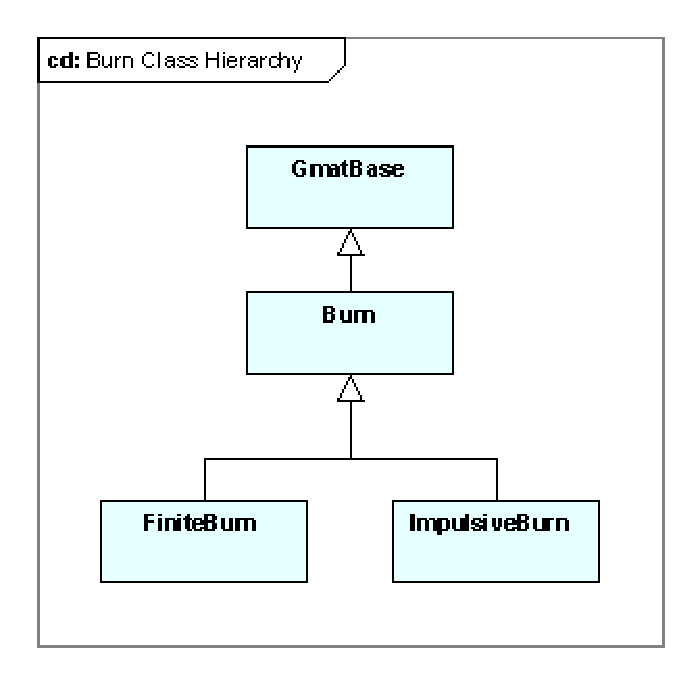
\includegraphics[scale=0.5]{Images/BurnClassHierarchy.eps}
\caption{\label{figure:BurnClassOverview}Class Hierarchy for Gmat's Burn Resources}
\end{center}
\end{figure}

The somewhat tedious descriptions provided above show the interfaces into parameters for the
configured objects in a static format.  The next two sections show in a bit more detail how these
interfaces are used to set parameters and to construct a serialized version of a GmatBase object. 
We'll begin with an example setting several properties on an ImpulsiveBurn object.  The class
hierarchy for ImpulsiveBurns is shown in Figure~\ref{figure:BurnClassOverview}.

\lstset{numbers=left,firstnumber=1,escapeinside={(*@}{@*)}}
\begin{lstlisting}[caption={Script Listing for an ImpulsiveBurn},
label={listing:ImpulsiveBurn}]
Create ImpulsiveBurn Burn1;

(*@\label{line:IBScriptFirstParameter}@*)Burn1.Origin = Earth;
Burn1.Axes = VNB;
Burn1.VectorFormat = Cartesian;
Burn1.Element1 = 3.16;
Burn1.Element2 = 0;
(*@\label{line:IBScriptLastParameter}@*)Burn1.Element3 = 0;
\end{lstlisting}
\lstset{numbers=none}

The serialized text -- that is, the scripting -- for an ImpulsiveBurn object is shown in
Listing~\ref{listing:ImpulsiveBurn}.  As can be seen on
lines~\ref{line:IBScriptFirstParameter}~--~\ref{line:IBScriptLastParameter} in this listing,
ImpulsiveBurn objects have six accessible parameters that users can manipulate: the Origin of the
burn (``Origin''), the Axes used to orient the burn in space (``Axes''), a format defining how the
burn is written relative to these axes (``VectorFormat''), and the three components necessary to
define the delta-V that this burn models (``Element1'', ``Element2'', and ``Element3'').

When GMAT reads a script containing these lines, it creates a new ImpulsiveBurn object named Burn1
and sets the values found in the script into the associated parameters on the object.  The object
creation process was described in Section~\ref{section:ObjectCreation}. 
Figure~\ref{figure:SettingBurnParameters} shows the calls made to the new object to set the
parameter values.  The steps shown in this figure are straightforward:

\begin{enumerate}
\item \textbf{Call Burn1->GetParameterType(``Origin'')} Determines that the ``Origin'' parameter
is a string.
\item \textbf{Call Burn1->SetStringParameter(``Origin'', ``Earth'')} Sets the ``Origin''
parameter to the string ``Earth''.
\item \textbf{Call Burn1->GetParameterType(``Axes'')} Determines that the ``Axes'' parameter
is a string.
\item \textbf{Call Burn1->SetStringParameter(``Axes'', ``VNB'')} Sets the ``Axes''
parameter to the string ``VNB'', denoting that the burn is specified in the
Velocity-Normal-Binormal representation.
\item \textbf{Call Burn1->GetParameterType(``VectorFormat'')} Determmines that the ``VectorFormat''
parameter is a string.
\item \textbf{Call Burn1->SetStringParameter(``VectorFormat'', ``Cartesian'')} Sets the
``VectorFormat'' parameter to the string ``Cartesian''.
\item \textbf{Call Burn1->GetParameterType(``Element1'')} Determines that the ``Element1'' parameter
is a Real number.
\item \textbf{Call Burn1->SetRealParameter(``Element1'', 3.16)} Sets the ``Element1''
parameter to the value 3.16.
\item \textbf{Call Burn1->GetParameterType(``Element2'')} Determines that the ``Element2'' parameter
is a Real number.
\item \textbf{Call Burn1->SetRealParameter(``Element2'', 0)} Sets the ``Element2''
parameter to the value 0.0.
\item \textbf{Call Burn1->GetParameterType(``Element3'')} Determines that the ``Element3'' parameter
is a Real number.
\item \textbf{Call Burn1->SetRealParameter(``Element3'', 0)} Sets the ``Element3''
parameter to the value 0.0.
\end{enumerate}

\begin{figure}[htb]
\begin{center}
\includegraphics[scale=0.5]{Images/SettingBurnParameters.eps}
\caption{\label{figure:SettingBurnParameters}Parameter Setting for
Listing~\ref{listing:ImpulsiveBurn}}
\end{center}
\end{figure}

\subsection{Serializing GmatBase Objects}

Objects are written to text using the GetGeneratingString() method.  GetGeneratingString can
serialize objects this way for several purposes: to write an object to a script file, to pass the
object to MATLAB or a MATLAB compatible external process, or in some cases to generate data used
for the generation of an ephemeris file.  The mode used for the serialization is determined using a
setting on the call to GetGeneratingString().  That setting, the write mode, is set using the
WriteMode enumeration.

The following paragraphs describe the process followed when performing serialization of GmatBase
objects.  We begin with a brief description of the WriteMode enumeration, followed by a detailed
description of the call to GetGeneratingString that serializes an object for scripting purposes,
and conclude with a description of the differences encountered when serializing an object for
MATLAB.

\subsubsection{\label{section:GenStringModes}The WriteMode Enumeration}

Table~\ref{table:WriteModeEnum} shows the modes available to the GetGeneratingString methods for
serialization of objects in GMAT.  These modes are defined in an enumeration, WriteMode, contained
in the Gmat namespace.  GMAT uses the SCRIPTING mode as the default write mode, generating text
strings that are designed to work with the script interpreter classes when saving a model to a
script file.

\begin{table}[htb]
\begin{center}
\caption{\label{table:WriteModeEnum}The WriteMode Enumeration}
\setlength\extrarowheight{2pt}
\begin{tabular}{|p{1.7in}|p{4in}|}
\hline
Identifier & Description \\
\hline
\hline
SCRIPTING & The mode used when writing an object as it appears in GMAT's script files.\\
SHOW\_SCRIPT & Similar to the SCRIPTING mode, the SHOW\_SCRIPT mode serializes an object as it
would appear in a script file.  The SHOW\_SCRIPT mode does not guarantee that the resulting text
is indented as it would be in a written script.\\
OWNED\_OBJECT & OWNED\_OBJECT mode is used to serialize the objects owned by an object that is
being written to the text stream.\\
MATLAB\_STRUCT & Generates the serialed object as a MATLAB structuire, so that the object can be
passed into MATLAB for external processing.\\
EPHEM\_HEADER & Generates a string used in GMAT's output ephemeris headers.\\
\hline
\end{tabular}
\end{center}
\end{table}

\subsubsection{Writing to Script}

\begin{figure}[htb]
\begin{center}
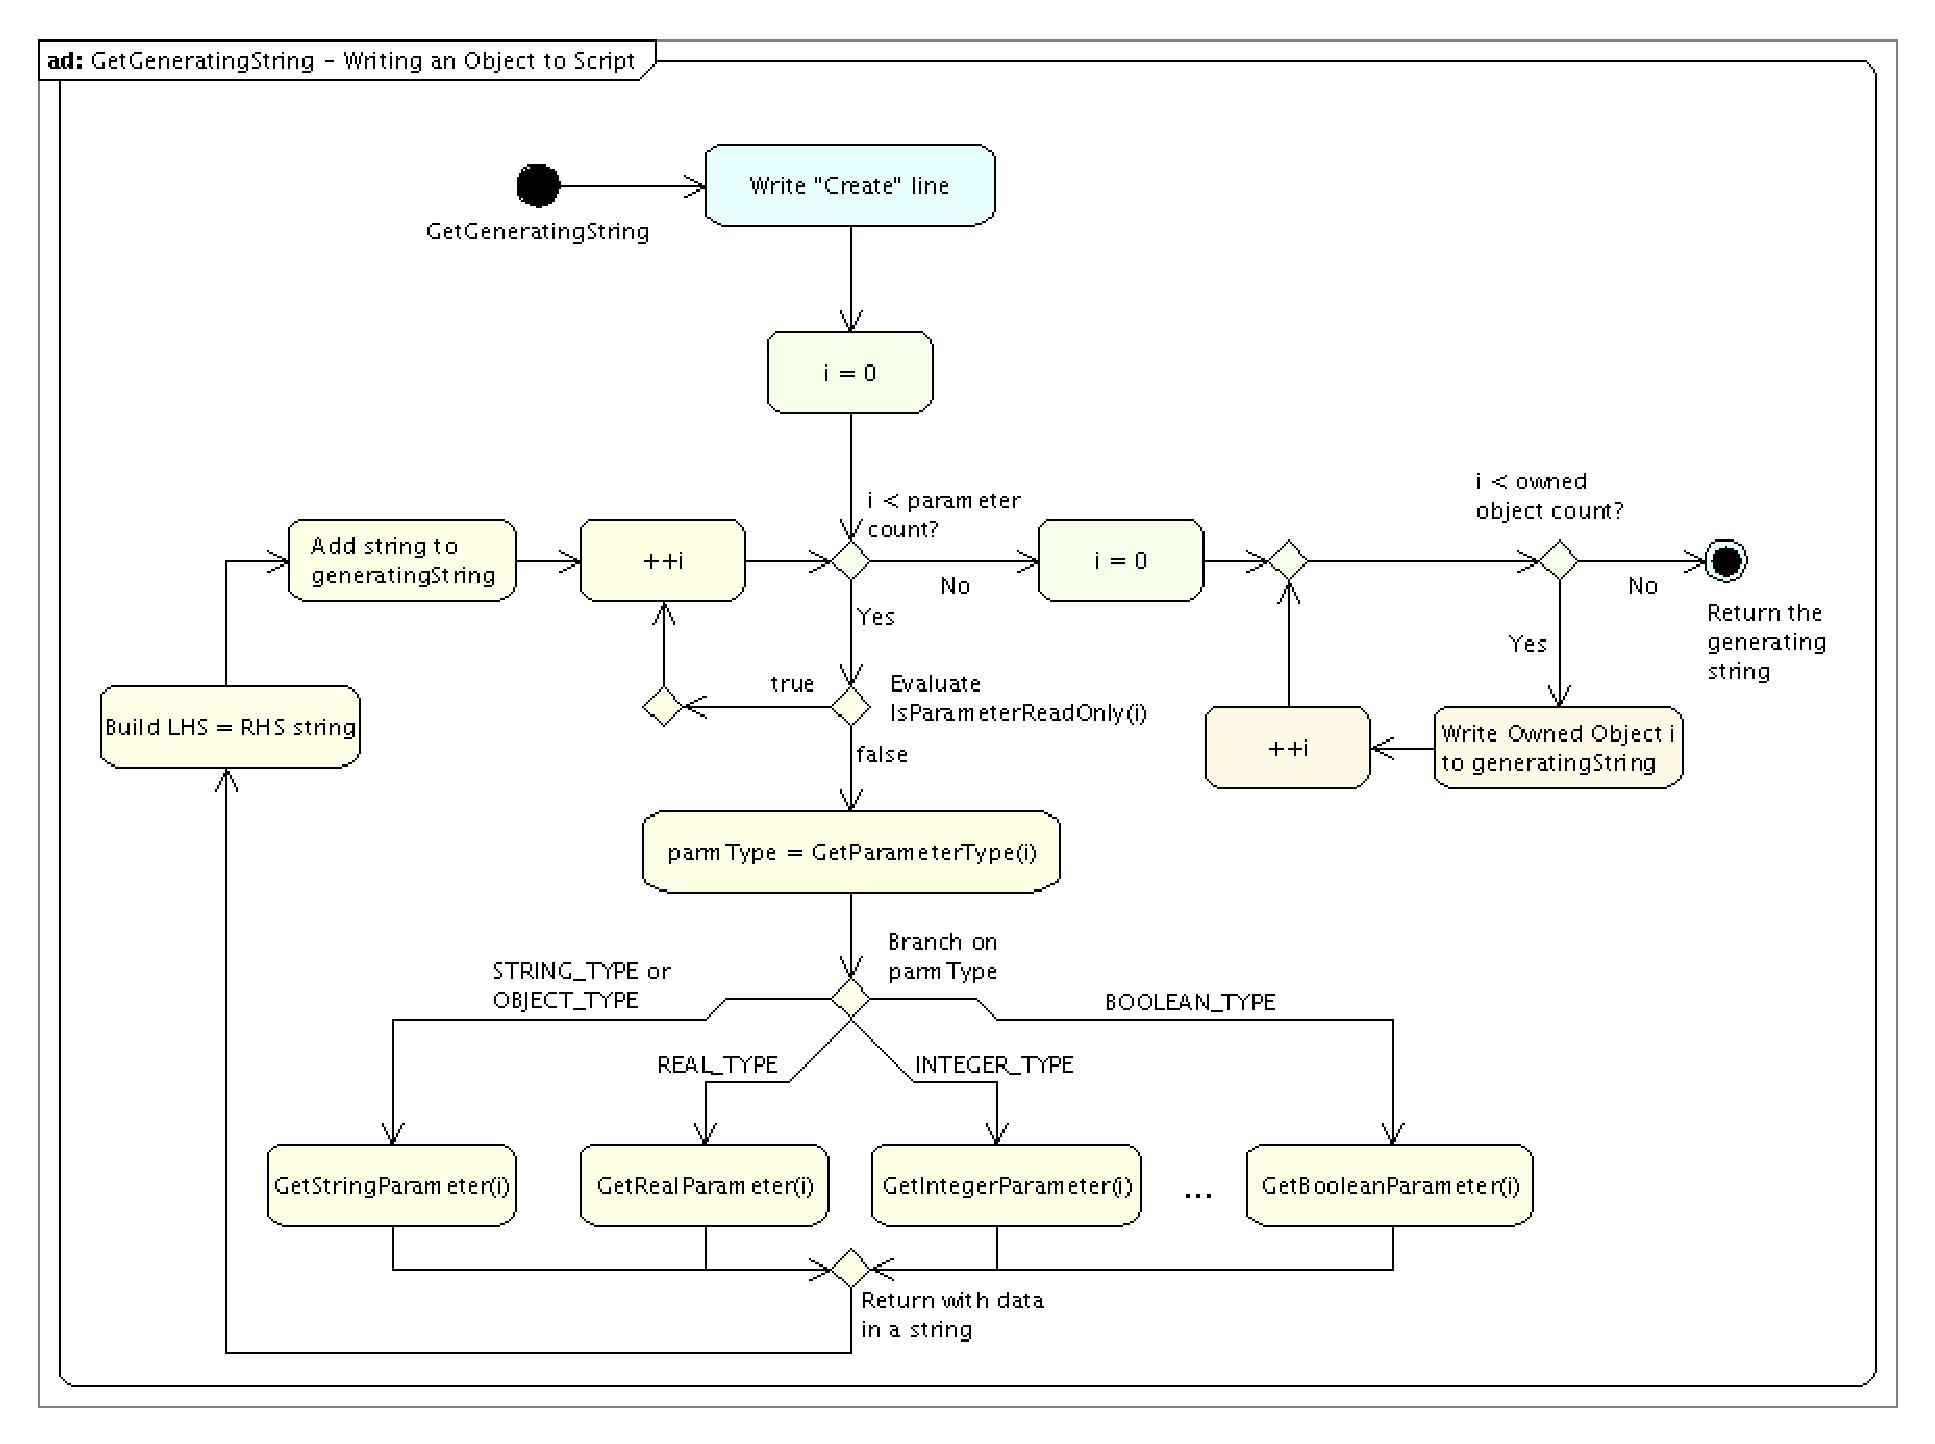
\includegraphics[scale=0.5]
{./Images/GetGeneratingStringWritinganObjecttoScript.eps}
\caption{\label{figure:GetGeneratingStringDetails}Flow in the GetGeneratingString() Method}
\end{center}
\end{figure}

Figure~\ref{figure:GetGeneratingStringDetails} shows the procedure followed when the
GetGeneratingString() method is called on a configured object to write that object in script
format\footnote{GetGeneratingString() can be overridden by the derived classes.  The description
provided here is the default behavior.  Command classes, in particular, always override this
method so that the command specific scripting can be generated.}. The process starts by clearing the
current generatingString attribute, and then writing the initial Create line to it.  Objects
without any parameters or owned objects are finished at this point, and simply return the resulting
string, following the path shown in green in the figure.

If the object's parameter count is not zero, then the GetGeneratingString() method calls the
WriteParameters() method, which adds text lines to the generatingString for each parameter that is
writable.  This process is shown in yellow in the figure.  The process starts by initializing an
index into the parameter list for the object.  This index is used to loop through the parameters
for the object.  For each parameter, the code calls the IsParameterReadOnly() method to determine
 if the parameter should be written to teh generating string.  If the parameter is not read only,
the current value of the parameter is sent into a string in the WriteParameterValue() method.  The
WriteParameterValue method determines the type of the parameter, and calls the corresponding access
method to retrieve the value and place it into a string.  This string is returned to the
WriteParameters() method for use as the right hand side of the text string setting the parameter's
value.  The parameter setting string is then build, using a call to GetParameterText() for the left
side of the parameter setting string and the string returned from the call to WriteParameterValue()
for the right side of the parameter setting string.  The resulting string is added to the
generating string, and the parameter index is incremented to move to the next parameter.

Once the parameter index has iterated through all of the parameters, the call to WriteParameters()
returns control to the GetGeneratingString() method.  GetGeneratingString() resets its index, and
then checks for owned objects.  If there are any owned objects, each owned object writes its data
to the generating string, following the process shown in orange in the figure.  Owned objects write
their data through calls to their GetGeneratingString() methods, with the write mode set to teh
OWNED\_OBJECT mode.  After all of the owned objects have been written, the generating string is
returned to the caller, completing the serialization process.

Listing~\ref{listing:CoordinateSystem} shown an example of the output generated when a coordinate
system is written to script.

\lstset{numbers=left,firstnumber=1,escapeinside={(*@}{@*)}}
\begin{lstlisting}[caption={Script Listing for a Coordinate System},
label={listing:CoordinateSystem}]
Create CoordinateSystem SunPointingCS;
GMAT SunPointingCS.Origin = DefaultSC;
GMAT SunPointingCS.Axes = ObjectReferenced;
GMAT SunPointingCS.UpdateInterval = 60;
GMAT SunPointingCS.OverrideOriginInterval = false;
GMAT SunPointingCS.XAxis = R;
GMAT SunPointingCS.ZAxis = N;
GMAT SunPointingCS.Primary = DefaultSC;
GMAT SunPointingCS.Secondary = Sun;
\end{lstlisting}
\lstset{numbers=none}

\subsubsection{Writing to MATLAB}

The process followed when an object is serialized for export to MATLAB is the same as that shown in
the sequence diagram for writing to script, Figure~\ref{figure:GetGeneratingStringDetails}.  The
key differences between the processes are contained in the details of the strings generated.  When
an object is serialized for MATLAB, the Create line is omitted.  The ``GMAT'' preface used for
parameter strings in SCRIPTING mode is also omitted, and strings are enclosed in single quotes to
conform to MATLAB's syntax.  Listing~\ref{listing:MATLABCoordinateSystem} shows the resulting
serailized version of the same coordinate system as was shown in the script serialization example,
above.

\lstset{numbers=left,firstnumber=1,escapeinside={(*@}{@*)}}
\begin{lstlisting}[caption={MATLAB Listing for a Coordinate System},
label={listing:MATLABCoordinateSystem}]
SunPointingCS.Origin = 'DefaultSC'
SunPointingCS.Axes = 'ObjectReferenced'
SunPointingCS.UpdateInterval = 60
SunPointingCS.OverrideOriginInterval = false
SunPointingCS.XAxis = 'R'
SunPointingCS.ZAxis = 'N'
SunPointingCS.Primary = 'DefaultSC'
SunPointingCS.Secondary = 'Sun'
\end{lstlisting}
\lstset{numbers=none}

\subsection{GmatBase Derivatives}

\begin{figure}[htb]
\begin{center}
\includegraphics[scale=0.5]{Images/GmatBaseSubclasses.eps}
\caption{\label{figure:GmatBaseSubclasses}Classes Derived from GmatBase}
\end{center}
\end{figure}

Figure~\ref{figure:GmatBaseSubclasses} shows the classes derived from GmatBase.  These classes are
presented more fully in other chapters of this document.  Here is a brief description of each, with
cross references to the chapters that provide the detailed descriptions:

\begin{description}
\item \textbf{AtmosphereModel} Models the Atmosphere for bodies in the SolarSystem.  The
AtmosphereModel classes are used to determine atmospheric densities in GMAT's Drag models.  Force
modeling is described in Chapter~\ref{chapter:ForceModel}.
\item \textbf{Attitude} The base class for attitude modeling in GMAT.  Attitude modeling is
described in Chapter~\ref{chapter:Attitude}.
\item \textbf{Burn} The base class for burn modeling.  The Burn class contains the elements common
to finite and impulsive burns.  The burn classes and other components used in maneuver modeling are
described in Chapter~\ref{chapter:Maneuvers}.
\item \textbf{CoordinateBase} The base class for coordinate system modeling.  GMAT provides a quite
extensive system of coordinate system models, described in Chapter~\ref{chapter:CoordinateSystems}.
\item \textbf{Function} The base class for internal and external functions, described in
Chapter~\ref{chapter:Functions}.
\item \textbf{GmatCommand} The base class for the commands in the Mission Control Sequence. 
Commands are described in Chapters~\ref{chapter:Commands} and~\ref{chapter:SpecificCommands}.
\item \textbf{Hardware} The base class for hardware elements that can be attached to other objects. 
Fuel tanks, thrusters, sensors, and antennae are all derived from this class.  THe Hardware classes
are described in Chapter~\ref{chapter:Hardware}.
\item \textbf{Interpolator} The base class for the numerical interpolaters.  The interpolators are
described in Chapter~\ref{chapter:Utilities}.
\item \textbf{MathNode} GMAT supports mathematics performed as part of the Mission Control
Sequence. Mathematical expressions are decomposed into a tree structure for evaluation.  The
MathNode class is used for the nodes in this tree structure, as is described in
Chapter~\ref{chapter:InlineMath}.
\item \textbf{MathTree} MathTree objects are used as containers for inline mathematicas in GMAT's
Mission Control Sequence, as is described in Chapter~\ref{chapter:InlineMath}.
\item \textbf{Parameter} GMAT can calculate many different properties that are useful for analyzing
spacecraft missions.  The code that implements these calculations is derived from the Parameter
class, described in Chapter~\ref{chapter:Parameters}.
\item \textbf{PhysicalModel} The PhysicalModel class is the base class for all of the forces used
in GMAT's propagators.  Force mdodeling is described in Chapter~\ref{chapter:ForceModel}.
\item \textbf{Propagator} The Propagator class is the base class for the numerical integrators and
analytic propagators\footnote{GMAT does not currently contain any analytic propagators; when such
propagators are added to the system, they will be derived from the Propagator class.} in GMAT. 
Propagators are described in Chapter~\ref{chapter:Propagators}.
\item \textbf{PropSetup} The PropSetup class is a container class that connects propagators to
force models.  When a user creates a ``Propagator'' in GMAT, the object that is created is really a
PropSetup instance.  The PropSetup class description is in Chapter~\ref{chapter:Propagators}.
\item \textbf{SolarSystem} The SolarSystem class is the container class used to hold all of the
elements of the space environment: stars, planets, moons, other celestial bodies, calculated
points, and any other entities that are used in the environment model.  The SolarSystem instances
include specification of global sources for the model as well -- for example, identification of the
planetary ephemeris souce used.  These elements are described in Chapter~\ref{chapter:SolarSystem}.
\item \textbf{Solver} Solver classes are used to drive targeting, optimization, and parametric
analysis tasks.  The Solvers are described in Chapter~\ref{chapter:Solvers}.
\item \textbf{SpacePoint} All objects that have a physical location in the solar system are derived
from the SpacePoint class.  This class is the base class for everything from elements of the solar
system to the spacecraft and groundstations.  The SpacePoint class is described in
Chapter~\ref{chapter:SolarSystem}.
\item \textbf{StopCondition} GMAT's integrators can stop when any of a large set of conditions is
met.  This ability to stop is provided through the stopping condition class, described in
Chapter~\ref{chapter:Parameters}.
\item \textbf{Subscriber} Subscribers are the recipients of data in GMAT's publish and subscribe
subsystem, introduced in Chapter~\ref{chapter:Publisher}.  The Subscriber base class, used for all
subscribers, is described in Chapter~\ref{chapter:Factories}.
\end{description}

\section{\label{section:Namespaces}Namespaces}

GMAT uses several namespaces defined for specific purposes.  The ``Gmat'' namespace is used to
define program specific enumerations defining the types of objects users can configure in GMAT, the
types of data structures commonly used in the system, and more specialized enumerations used by
some of GMAT's subsystems.

\section{\label{section:Enumerations}Enumerations}

GMAT uses enumerations to identify some of the key types of objects and parameters in the system,
the current state of the system, and to track modes for some of the system processes.  The
remainder of this chapter tabulates the enumerations that are not listed in other places in this
document.

\subsection{The ParameterType Enumeration}

GmatBase includes a method, GetParameterType(id), which returns an integer identifier for the type
of the parameter with the ID input to the function.  The return value is a member of the
ParameterType enumeration, defined in the Gmat namespace.  This enumeration is described in
Table~\ref{table:ParameterTypeEnum}.

\begin{table}[htb]
\begin{center}
\caption{\label{table:ParameterTypeEnum}The ParameterType Enumeration}
\setlength\extrarowheight{2pt}
\begin{tabular}{|p{2.5in}|p{3.2in}|}
\hline
Identifier & Description \\
\hline
\hline
INTEGER\_TYPE & Integer parameters \\
UNSIGNED\_INT\_TYPE & Unsigned integer paramneters.\\
UNSIGNED\_INTARRAY\_TYPE & Arrays of unsigned integers.\\
REAL\_TYPE & Real numbers.\\
REAL\_ELEMENT\_TYPE & A Real number accessed from an array.\\
STRING\_TYPE & A string.\\
STRINGARRAY\_TYPE & A vector of strings.\\
BOOLEAN\_TYPE & A boolean value that evaluates to tru or false.\\
RVECTOR\_TYPE & An Rvector\\
RMATRIX\_TYPE & An Rmatrix\\
TIME\_TYPE & A Real used to represent time.\\
OBJECT\_TYPE & An object.\\
OBJECTARRAY\_TYPE & A vector of objects.\\
ON\_OFF\_TYPE & A boolean that evaluates to either ``On'' or ``Off''\\
TypeCount & The totla number of ParameterTypes available. \\
UNKNOWN\_PARAMETER\_TYPE & Unknown parameter types.\\
& Set to -1. \\
\hline
\end{tabular}
\end{center}
\end{table}


\subsection{\label{section:WrapperDataTypeEnum}The WrapperDataType Enumeration}

Some components of GMAT need to access data elements in a generic fashion.  These components, most
notably including the Command subsystem, use a class of wrapper objects that take the disparate
types and present a common interface into those types.  The WrapperDataType enumeration is used to
identify the type of underlying object presented by the wrapper classes.  More information about
this object can be found in Section~\ref{section:DataWrappers}.  The defined wrapper types used in
this enumeration are shown in Table~\ref{table:WrapperDataTypeEnum}.

\begin{table}[htb]
\begin{center}
\caption{\label{table:WrapperDataTypeEnum}The WrapperDataType Enumeration}
\setlength\extrarowheight{2pt}
\begin{tabular}{|p{1.7in}|p{4in}|}
\hline
Identifier & Description \\
\hline
\hline
NUMBER & a Real or Integer value entered explicitly into the command \\
STRING & a text string with no associated object \\
OBJECT\_PROPERTY & an internal data member of an object, accessible using the GmatBase
parameter accessor methods (GetRealParameter(), GetIntegerParameter(), etc) \\
VARIABLE & an instance of the Variable class \\
ARRAY & an instance of the Array class \\
ARRAY\_ELEMENT & an element of an Array object \\
PARAMETER\_OBJECT & any other object derived from the Parameter class \\
\hline
\end{tabular}
\end{center}
\end{table}


\subsection{The ObjectType Enumeration}

GMAT has an enumeration in the Gmat namespace designed to provide ID values for each of the core
types used in the system.  Table~\ref{table:ObjectTypeEnum} shows the identifiers for each entry in
this enumeration, along with a brief description of the type of object the entry identifies.

\begin{table}[htb]
\begin{center}
\caption{\label{table:ObjectTypeEnum}The ObjectType Enumeration}
\setlength\extrarowheight{2pt}
\begin{tabular}{|p{1.68in}|p{2.5in}|p{1.65in}|}
\hline
Identifier & Objects Identified & Notes \& References \\
\hline
\hline
SPACECRAFT & Spacecraft & Initialized to 1001\\ & & Chapter~\ref{chapter:Spacecraft} \\
FORMATION & Formations & Chapter~\ref{chapter:Spacecraft} \\
SPACEOBJECT & Spacecraft and Formations & Chapter~\ref{chapter:Spacecraft} \\
GROUND\_STATION & Groundstations & Not yet used \\
BURN & Burn objects for finite and impulsive maneuvers & Chapter~\ref{chapter:Maneuvers} \\
COMMAND & Commands in the Mission Control Sequence & Chapters~\ref{chapter:Commands}
and~\ref{chapter:SpecificCommands} \\
PROPAGATOR & Propagators and Integrators & Chapter~\ref{chapter:Propagators} \\
FORCE\_MODEL & Force Models & Chapter~\ref{chapter:ForceModel} \\
PHYSICAL\_MODEL & Individual Forces & Chapter~\ref{chapter:ForceModel} \\
TRANSIENT\_FORCE & Forces that are dynamically added or removed & Chapter~\ref{chapter:Maneuvers} \\
INTERPOLATOR & Interpolators & Chapter~\ref{chapter:Utilities} \\
SOLAR\_SYSTEM & Solar System & Chapter~\ref{chapter:SolarSystem} \\
SPACE\_POINT & Objects that have physical locations in the Solar System &
Chapter~\ref{chapter:SolarSystem} \\
CELESTIAL\_BODY & Stars, Planets, and Moons & Chapter~\ref{chapter:SolarSystem} \\
CALCULATED\_POINT & Barycenters and Libration Points & Chapter~\ref{chapter:SolarSystem} \\
LIBRATION\_POINT & Libration Points & Chapter~\ref{chapter:SolarSystem} \\
BARYCENTER & Barycenters & Chapter~\ref{chapter:SolarSystem} \\
ATMOSPHERE & Atmosphere Models & Chapter~\ref{chapter:ForceModel} \\
PARAMETER & Calculated Parameters, Variables, and Arrays & Chapter~\ref{chapter:Parameters} \\
STOP\_CONDITION & Stopping Conditions & Chapter~\ref{chapter:Parameters} \\
SOLVER & Targeters, Optimizers, and Scanners & Chapter~\ref{chapter:Solvers} \\
SUBSCRIBER & Subscribers & Chapter~\ref{chapter:Factories} \\
PROP\_SETUP & PropSetups & Chapter~\ref{chapter:Propagators} \\
FUNCTION & Internal or External Functions & Chapter~\ref{chapter:Functions} \\
FUEL\_TANK & Fuek Tanks & Chapter~\ref{chapter:Hardware} \\
THRUSTER & Thrusters & Chapter~\ref{chapter:Hardware} \\
HARDWARE & Tanks, Thrusters, Antennae, Sensors, etc.  & Chapter~\ref{chapter:Hardware} \\
COORDINATE\_SYSTEM & Coordinate Systems & Chapter~\ref{chapter:CoordinateSystems} \\
AXIS\_SYSTEM & Axis Systems & Chapter~\ref{chapter:CoordinateSystems} \\
ATTITUDE & Attitude & Chapter~\ref{chapter:Attitude} \\
MATH\_NODE & Elements of Equations & Chapter~\ref{chapter:InlineMath} \\
MATH\_TREE & Parsed Mathematical Equations & Chapter~\ref{chapter:InlineMath} \\
UNKNOWN\_OBJECT & Objects that are not otherwise identified & Objects without one of the types
listed above \\
\hline
\end{tabular}
\end{center}
\end{table}

\subsection{The RunState Enumeration}

The GMAT engine is always maintained in a specific state while the system is running, as is
described in Section~\ref{section:ModeratorStates}.  The RunState enumeration, tabulated in
Table~\ref{table:RunStateEnum} is used to track these states.

\begin{table}[htb]
\begin{center}
\caption{\label{table:RunStateEnum}The RunState Enumeration}
\setlength\extrarowheight{2pt}
\begin{tabular}{|p{1.7in}|p{4in}|}
\hline
Identifier & Description \\
\hline
\hline
IDLE & Initialized to 10000.  The IDLE state indicates that GMAT's engine is waiting for
instructions from the user.\\
RUNNING & GMAT enters the RUNNING state when the user starts a mission run.\\
PAUSED & When the user presses the Pause button on the GUI, GMAT enters the PAUSED state.\\
TARGETING & GMAT enters the TARGETING state when the Mission Control Sequence enters a Target
loop.\\
OPTIMIZING & GMAT enters the TARGETING state when the Mission Control Sequence enters an Optimize
loop.\\
SOLVING & GMAT enters the TARGETING state when the Mission Control Sequence enters other solver
loops.\\
WAITING &  GMAT defines the WAITING state for use when waiting for completion of an external
process.  The current code does not use the WAITING state.\\
\hline
\end{tabular}
\end{center}
\end{table}


